\documentclass{article}

% if you need to pass options to natbib, use, e.g.:
\PassOptionsToPackage{numbers, compress}{natbib}
% before loading nips_2017
%
% to avoid loading the natbib package, add option nonatbib:
% \usepackage[nonatbib]{nips_2017}

%\usepackage{nips_2017}

% to compile a camera-ready version, add the [final] option, e.g.:
\usepackage[final]{nips_2017}

\usepackage[utf8]{inputenc} % allow utf-8 input
\usepackage[T1]{fontenc}    % use 8-bit T1 fonts
\usepackage{hyperref}       % hyperlinks
\usepackage{url}            % simple URL typesetting
\usepackage{booktabs}       % professional-quality tables
\usepackage{amsfonts}       % blackboard math symbols
\usepackage{nicefrac}       % compact symbols for 1/2, etc.
\usepackage{microtype}      % microtypography
\usepackage{algorithm}
\usepackage[noend]{algpseudocode}
\usepackage{shortcuts}
\usepackage{bm}
\usepackage[dvipsnames]{color}
\usepackage{amsmath,amsthm,amssymb,parskip,setspace,tabularx, wrapfig,float,enumerate} 
\usepackage{tikz, setspace, subfig, grffile}
\usepackage{subfig}
\usetikzlibrary{bayesnet}

\title{Mapping Gaussian Process Priors
\\ to Bayesian Neural Networks}

% The \author macro works with any number of authors. There are two
% commands used to separate the names and addresses of multiple
% authors: \And and \AND.
%
% Using \And between authors leaves it to LaTeX to determine where to
% break the lines. Using \AND forces a line break at that point. So,
% if LaTeX puts 3 of 4 authors names on the first line, and the last
% on the second line, try using \AND instead of \And before the third
% author name.

\author{
  Daniel Flam-Shepherd \\
  University of Toronto \\
  %\texttt{ @cs.cranberry-lemon.edu} \\
  \And
  James Requeima  \\
  University of Cambridge \\
  % \texttt{email} \\
  \AND
  David Duvenaud \\
  University of Toronto \\
  %% Address \\
  %% \texttt{email} \\
}

\begin{document}
% \nipsfinalcopy is no longer used

\maketitle


\begin{abstract}
This paper describes a method to "map" a Gaussian process prior to a Bayesian Neural Net.
This is done by minimizing over some data distribution of interest the kullback leibler
divergence from prior distributions of the Gaussian process to the Bayesian Neural Net
(in function space). This allows of to train a Bayesian Neural Net with apriori knowledge
of the covariance structure of the data distribution in the input space. 
\end{abstract}

\section{Introduction and Motivation}

What defines a reasonable prior to use when forming and training Bayesian models 
and Bayesian neural networks? In a recent work, (Ghosh et al 2016) 
apply a horseshoe prior over preactivations of a Bayesian neural network to 
effectively turns off weights that do not help explain the data. That model and 
many Bayesian models view priors solely in parameter space, in this work we move 
forward with viewing priors in function space as well. 

It is difficult to incorporate meaningful prior information about functions to be modelled by BNNs since priors are generally specified over the network parameters. Often, normal distributions are placed over the weights for convenience and are interpreted as a bias toward less complex functions via smaller weights. Gaussian processes, on the other hand, have a elegant mechanism for incorporating prior beliefs about the underlying function - specifying the mean and covariance functions. However, Gaussian Process have scalability limitations making bayesian neural networks a more practical model in large data settings. In our work, we present an approach to specify a more principled prior for Bayesian Neural Networks that can leverage the well studied kernel design techniques from Gaussian process regression.


We consider matching the prior of a Bayesian neural network $\pbnn (\bm f |\bm \phi )$
to the prior of a Gaussian process $\pgp (\bm f | \bm \theta ) $ 
 by minimizing their KL divergence over 
some data distribution of interest $\X \sim p(\X)$. 
We minimize the KL divergence with respect to the initial variational parameters $\bm \phi$ 
of the proposal distribution $q(\B w |\bm \phi)$. 
These variational parameters 
$\bm \phi^* = \{ \bm \mu _{\bm \phi}^* , \log \bm \sigma _{\bm \phi} ^* \} $ 
yield a prior on the BNN weights 
$p(\B w) = \N (\B w |\bm \mu _{\bm \phi}^* , \bm \sigma _{\bm \phi} ^* )\equiv q(\B w | \bm \phi ^*)$. 
Then, variational inference allows us to perform approximate inference in our BNN using this more 
principled prior. In both stochastic optimization steps, we use the reparameterization trick \citet{vae} to sample from the weights $\B w$ and draw functions from our BNN. 
We describe the implementation of both steps in the next section. 


\begin{figure}[h]\centering
\subfloat[BNN ]{\centering
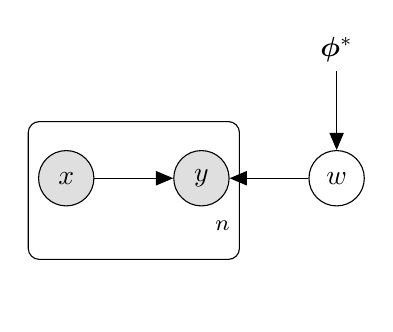
\begin{tikzpicture}[-latex, auto, l/.style={draw,thick,dashed}]
  \node[obs]                               (x) {$\B  x $};
  \node[below=of x]                               (s) {};
  \node[obs, right=of x]                   (y) {$\B  y $};
  \node[latent,right= of y]            (w) {$\B w$};
  \node[above= of w]                    (t) {$\bm \phi ^*$};
  

  % Connect the nodes
  \edge{x}{y};
  \edge{t}{w};
  \edge{w}{y};
  %\path[l] (x) edge [ bend left =40]node[left] {} (f);
        
  % Plates
  \plate[minimum size=1.75cm] {} {(x)(y)} {$n$} ;
\end{tikzpicture}
}
\hspace*{2.5cm}
\subfloat[GP ]{\centering
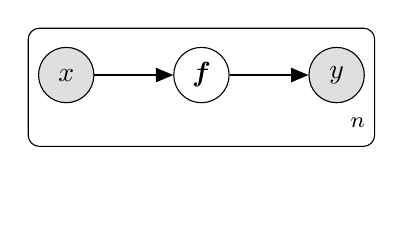
\begin{tikzpicture}[-latex, auto, l/.style={draw,thick,dashed}]
  \node[obs]                               (x) {$\B  x $};
  \node[below=of x]                               (s) {};
  \node[latent, right=of x]                (f) {$\bm f$};
  \node[obs, right=of f]                   (y) {$\B  y $};


  % Connect the nodes
  \edge{x}{f};
  \edge{f}{y};
   \plate[minimum size=1.5cm] {} {(x)(y)} {$n$} ;
 \end{tikzpicture}
}
\caption{ (a) and (b) display the graphical models of a BNN and GP.
} \label{fig:1}
\end{figure}

\subsection{Contributions}
\begin{itemize}
    \item We formulate two methods to map the prior of a Gaussian process to a Bayesian neural network 
          working strictly in function space. The first minimizes the distributions over functions of 
          the BNN to the GP. The second trains in adversarial fashion a BNN prior to generate functions
          from a data distribution that resemble functions sampled from a GP prior.
    \item We provide an stochastic optimization algorithm for the implementation of both methods using the
          reparametrization trick.  
    \item We describe how to do kernel hyperparameter optimization within our formalism using 
          continuous methods that directly and indirectly optimize the log marginal likelihood (TO DO)
    \item We test our methods in a variety of toy regression tasks using synthetic data and (TO DO)
          some selected datasets from the UCI repository. 
    
\end{itemize}

\newpage

\section{Background on BNNs and GPs}

\subsection{Bayesian Neural Networks}
To do inference in BNN model we learn a variational approximation $q(\B w |\bm \varphi )$ to 
$ p(\B w | \D )$ the posterior distribution of the parameters $\B w$ conditioned on training data 
$\D =\{\B x_i,  \B y_i\}_{i=1}^N $ 
where $p(\B w |\D)= p(\D |\B w) p(\B w) / p(\D) $ 
where  $ p(\D) =\int p(\D |\B w) p(\B w) d\B w $
Learning the posterior on the parameters will mean updating our prior from 
$\B w \sim p(\B w)$ to $\B w \sim p(\B w|\D)$ as a consequence of the evidence from the training data     
$ \{\B x_i,  \B y_i\}_{i=1}^N \sim p(\D ) $. 
This distribution $\ap $ allows us to form a predictive distribution by integrating out $\B w$.
\[p(\by  | \B x, \D ) = \int p(\by | \B x, \B w) p(\B w | \D )d\B w = \E_{\ap}[p(\by | \B x, \B w)] \]
In SVI, we use the reparametrization trick to obtain a stochastic optimization problem on the parameters 
$\bphi$ of $\aq$ through minimizing the KL divergence $\kl [ \aq |\ap   ]$ or maximizing the 
evidence lower bound (ELBO) $\elbo (\bphi)$ of the marginal likelihood of the data:
\eqn{ \bm \phi^*  = \argmin{\bm \phi} \ \kl [ \aq |\ap   ] = \argmax{\bm \phi} \ \elbo _\D (\bm \phi) }
where $\elbo _\D (\bphi) = \E _{\aq}[\log p(\D|\B w] - \kl [ \aq | p(\B w)  ]  $


\subsection{Gaussian Processes}
A Gaussian process is a collection of random variables, any finite number of which have a joint Gaussian distribution.
A Gaussian process is completely specified by its mean and covariance function; $f(\B x) \sim  \gp (\mf , \kf ) $ 
\begin{align}
    \mf =\E[f(\B x)], \ \text{ and } \ k(\B x , \B x') = \E[(f(\B x)-m(\B x))(f(\B x')-m(\B x'))]
\end{align}

choose some subset of inputs $\B X _\bullet =\{\B x_i \}$ 
and write $\B K _{\bullet\bullet}= [k(\B x  ,\B x' )]$
Then we generate a random Gaussian vector with this covariance matrix via 
$\bm f  \sim \N (\B 0, \B K_{\bullet\bullet})$
The joint prior distribution of the training outputs, 
$\bm f= f(\B X_\bullet)$, and the test outputs $\bm f_*=f (\B X_*)$ 
according to the prior is
\[( \bm f , \bm f _* ) \sim \N (\B 0, \B C), \ \  \B C =\begin{pmatrix} \B K & \B K_{\bullet *} \\ \B K_{*\bullet} & \B K_{**} \end{pmatrix} \]

We can think of the formulation of GP as  generating functions
from the prior, and rejecting the ones that disagree with the observations. 
This corresponds to conditioning
the joint Gaussian prior distribution on the observations .

For predicting noisy targets $\B y = \bm f + \bm \epsilon $ 
where $\bm \epsilon \sim \N (\B 0 , \sd _n \I) $ 
where $\covar(\B y ) = \B K +\sd _n \I \equiv \B K_y$ so that 
we can write the joint distribution of 
the observed target values and the function values 
at the test locations under the prior as 
$ (\B y , \bm f_*) \sim \N (\B 0, \B C_*) $ where $\B C_*$ replaces $\B K $ with $\B K_{\B y}$. 
The predictive distribution is 
$p(\bm f_* | \B X_* , \B y, \B X_\bullet ) =\N (\E [\bm f_* ], \covar (\bm f_*))$ where
\begin{align*}
\E [\bm f_* ] =  \B K_{\bullet *} \B K_{\B y} ^{-1} \B y  , 
\ \text{ and } \  
\covar (\bm f_*) =  \B K_{**} -\B K_{*\bullet } \B K_{\B y}^{-1}\B K_{\bullet *}
\end{align*} 

\newpage

\section{ Step One : Learning the prior parameters by Minimizing the KL}
In this section we describe the procedure used to minimize the KL divergence of  
the BNN prior distribution over functions $\pbnn (\bm f |  \bm \phi ) $ and
the GP prior distribution over functions  $\pgp (\bm f | \bm \theta )$ 
where $\bm \theta$ are hyperparameters of the kernel $\B K$. 
\begin{align}
    \mathcal K_\X (\bm \phi)&= 
    \kl [\pbnn (\bm f |  \bm \phi ) \mid   \pgp (\bm f | \bm \theta )] 
    = \int\pbnn (\bm f |  \bm \phi ) \log \BB{\frac{\pbnn (\bm f |  \bm \phi ) }{   \pgp (\bm f | \bm \theta )}} d\bm f  \\
    &= -\entropy [\pbnn (\bm f |  \bm \phi ) ] 
       - \E_{\pbnn (\bm f |  \bm \phi ) } [\log \pgp (\bm f | \bm \theta ) ] 
    \propto -\frac{1}{S} \sum_{s=1}^S \log \pgp (\bm f ^{(s)}| \bm \theta ) 
\end{align}

Where we have used a Monte Carlo estimate of 
$ \E_{\pbnn (\bm f |  \bm \phi ) } [\log \pgp (\bm f | \bm \theta ) ]$, 
using S samples $ \bm f ^{(s)} \sim  \pbnn (\bm f |  \bm \phi )$.
We also assume that the entropy term $\entropy [\pbnn (\bm f |  \bm \phi ) ]$ 
is not a function of the variational parameters $\bm \phi$.
We define our first stochastic optimization objective by approximating the KL divergence between these infinite dimensional distributions by taking expectations over where $p(\X)$ allows us to prioritize where in the input space we want 
$\pbnn (\bm f |  \bm \phi ) \sim \pgp (\bm f | \bm \theta ) $
\begin{align}
     \elbo _\X (\bm \phi)
     &\equiv \E _{\X \sim p(\X)} [\mathcal K_\X (\bm \phi) ]
     \propto - \frac{1}{S} \sum_{s=1}^S  \E_{p(\B X)} [\log \pgp (\bm f ^{(s)}(\B x)| \bm \theta )] 
\end{align}

We minimize (3) $ \bm \phi ^* =  \amin{\bm \phi}  \elbo _\X (\bm \phi ) $.
This is described in Algorithm 1. 

\begin{algorithm}
\caption{Learn the prior}
\begin{algorithmic}[1]
\State \textbf{Initialize} $\bm \phi =\{ \bm \mu _{\bm \phi} , \log \bm \sigma _{\bm \phi}  \}$
\While{ $\bm \phi$ not converged}
    \State $ \bm \epsilon ^{(s)} \sim p(\bm \epsilon) = \N (\B 0, \I) $
    \Comment{sample prior noise}
    \State $\B w ^{(s)} \gets \bm g(\bm \phi, \bm \epsilon^{(s)}) = \bm \mu _{\bm \phi} + \bm \sigma _{\bm \phi}\bm \epsilon ^{(s)}$
    \Comment{sample $S$ weights $\B w \sim q(\B w | \phi) $}
    \State $\X \gets \{ \B x_1, \dots , \B x_n \sim p(\B x)\}$ 
    \Comment{sample data} 
    \State $\bm f ^{(s)} \gets   f(\B X , \B w^{(s)} )$ 
    \Comment{sample $S$ functions $\bm f \sim \pbnn (\bm f |  \bm \phi )$}
    \State $ \elbo _{\X} ( \bm \phi ) \gets   -\frac{1}{S} \sum_s \log \pgp (\bm f ^{(s)}| \bm \theta ) $
    \Comment{compute the kl}
    \State   $\nabla _{\bm \phi} \elbo _{\tiny \X} (\bm \phi )\gets -\frac{1}{S} \sum_s \nabla _{\bm \phi}\log \pgp (\bm f ^{(s)}| \bm \theta ) $
    \Comment{compute gradients of the kl}
    \State $\bm \phi \gets \text{adam}(\bm\phi ,\nabla _{\bm \phi} \elbo _{\tiny \X} (\bm \phi ) )$
    \Comment{update the parameters}
\EndWhile
\State \textbf{Return} $\bm \phi^*$
\end{algorithmic}
\end{algorithm}

\newpage 

\section{ Step One : Learning the prior parameters by an Adversarial Strategy}


In this section we describe an adversarial procedure used to map   
the BNN prior distribution over functions $\pbnn (\bm f |  \bm \phi ) $ to the 
the GP prior distribution over functions  $\pgp (\bm f )$. 
We treat the Bayesian neural network as the generator 
$G(\X , \B w ) =  f _{ \text{\tiny BNN}}(\X ; \bm t(\bm \phi, \bm \epsilon)  ) =\bm f _{ \text{\tiny BNN}}$ 
and define a parametric neural network discriminator $D(\bm f , \bm \theta_d )$ that 
takes in samples of functions from the Gaussian process prior and 
Bayesian neural net 'generator' and uses parameters $ \bm \theta_d $ to map
them to a scalar : the probability
that $\bm f$ came from $\pgp (\bm f )$  rather than $\pbnn (\bm f )$.
\begin{align}
    \mathcal V (\bm \phi_G, \bm \theta_D)&= 
    \E_{\bm f \sim \pgp (\bm f )}\BB{\log D(\bm f) } +
    \E_{\bm f \sim \pbnn (\bm f |  \bm \phi ) }  \BB{ \log (1- D(\bm f))  } \\
    &= \int \pgp (\bm f ) \log D(\bm f) d\bm f +  
       \int \pbnn (\bm f |  \bm \phi ) \log (1- D(\bm f)) d\bm f  \\
    &\approx \frac{1}{S} \sum_{s=1}^S \log D (\bm f ^{(s)}_{ \text{\tiny GP}} ) +
             \frac{1}{S} \sum_{s=1}^S \log (1-D (\bm f ^{(s)}_{ \text{\tiny BNN}} ) )
\end{align}

Where we have used Monte Carlo estimates of 
$\E _{\bm f \sim \pbnn (\bm f |  \bm \phi ) }  \BB{ \log (1- D(\bm f))  } $ and \\
$\E_{\bm f \sim \pgp (\bm f )}\BB{\log D(\bm f) } $ using S samples from 
$ \bm f ^{(s)}_{ \text{\tiny BNN}} \sim  \pbnn (\bm f)$ and 
$\bm f ^{(s)}_{ \text{\tiny GP}} \sim \pgp (\bm f )$

We define the stochastic optimization objective by approximating 
$ \mathcal V_\X (\bm \phi_G, \bm \theta_D)$ 
by taking expectations over where $p(\X)$ allows us to prioritize where in the input space we want 
$\pbnn (\bm f |  \bm \phi ) \sim \pgp (\bm f | \bm \theta ) $ ie 
$\mathcal V _\X (\bm \phi_G, \bm \theta_D) 
= \E _{\X \sim p(\X)} \BB{\mathcal V (\bm \phi_G, \bm \theta_D)}$
\begin{align}
     \mathcal V _\X (\bm \phi_G, \bm \theta_D)
     &\approx  \frac{1}{S} \sum_{s=1}^S  \E_{\X \sim p(\X)} 
     \BB{\log D (\bm f ^{(s)}_{ \text{\tiny GP}} (\X) ) 
     +\log \bb{ 1-D (\bm f ^{(s)}_{ \text{\tiny BNN}} (\B X) )}  } 
\end{align}

We will find 
$ (\bm \phi ^*_g , \bm \theta ^*_d) =  
\amin{\bm \phi} \argmax{\bm \theta }\ \mathcal V _\X (\bm  \phi_g, \bm \theta_d)  $. 
This is described in Algorithm 2. 

\begin{algorithm}
\caption{Learn the prior through an adversarial algorithm}
\begin{algorithmic}[1]
\State \textbf{Initialize} $\bm \phi =\{ \bm \mu _{\bm \phi} , \log \bm \sigma _{\bm \phi}  \}$ 
and $\bm \theta _D$
\While{ $\bm \phi$ not converged}
    \State $ \bm \epsilon ^{(s)} \sim p(\bm \epsilon) = \N (\B 0, \I) $
    \Comment{sample prior noise}
    \State $\B w ^{(s)} \gets \bm t(\bm \phi, \bm \epsilon^{(s)}) = \bm \mu _{\bm \phi} + \bm \sigma _{\bm \phi} \odot \bm \epsilon ^{(s)}$
    \Comment{sample $S$ weights $\B w \sim q(\B w |\bm \phi) $}
    \State $\X \gets \{ \B x_1, \dots , \B x_n \sim p(\B x)\}$ 
    \Comment{sample data} 
    \State  $\bm f ^{(s)}_{ \text{\tiny GP}} \gets   \B L \bm \epsilon ^{(s)} $ 
    \Comment{sample S function from the GP prior : 
             $\bm f ^{(s)}_{ \text{\tiny GP}} \sim \pgp (\bm f )$}
    \State $\bm f ^{(s)}_{ \text{\tiny BNN}} \gets   G(\B X ; \B w^{(s)} )$ 
    \Comment{sample $S$ functions from the BNN prior :
            $\bm f ^{(s)}_{ \text{\tiny BNN}} \sim  \pbnn (\bm f)$}
    \State $\B g _{\bphi } \gets \nabla _{\bphi } \mathcal V _\X (\bm \phi , \bm \theta_d)  $
    \Comment{compute the gradients of the BNN 'generator'}
    \State $\bm \phi \gets \text{adam}(\bm\phi ,\B g )$
    \Comment{update the BNN 'generator' parameters}
    \State $\B g _{\bm \theta _d} \gets \nabla _{\bm \theta _d } \mathcal V _\X (\bm \phi , \bm \theta_d)  $
    \Comment{compute the gradients of the discriminator}
    \State $\bm \theta_d \gets \text{adam}(\bm\phi ,\B g_{\bm \theta _d} )$
    \Comment{update the discriminator parameters}
\EndWhile
\State \textbf{Return} $\bm \phi^*$
\end{algorithmic}
\end{algorithm}





\newpage

\section{Step Two Maximize the Evidence Lower Bound}

Next, we use $\bm \phi^*$ found from step 1 to form a prior on the weights  
$p(\B w) =\N ( \B w |  \bm \mu _{\bm \phi} ^*,  \bm \sigma _{\bm \phi}^*)\equiv q(\B w | \bm \phi^*)$. 
Thereafter we learn the parameters 
$\bm \varphi =\{ \bm \mu_{\tiny\bm \varphi} , \log \bm \sigma _{\tiny \varphi} \} $
of the variational approximation 
$q(\B w | \bm \varphi) = \N (\B w |\bm \mu_{\tiny\bm \varphi} , \bm \sigma _{\tiny \varphi} )$ 
to the true posterior on the weights $p(\B w |\D )$. 
To do this we optimize the evidence lower bound (ELBO) $\elbo (\bm \varphi )$ 
with our optimized prior $p(\B w ) = q (\B w | \bm \bphi^*   ) $ 
\begin{align}
    \elbo _\D (\bm \varphi ) 
    &=  \E _{q (\B w | \bm \varphi)} \BB{ \log p (\D | \B w ) }  - 
        \kl [q (\B w | \bm \varphi) || q (\B w | \bm \bphi^*  ) ] \\ 
    &=  \entropy [ q (\B w | \bm \varphi)] + 
        \E _{q (\B w | \bm \varphi)} \BB{ \log p (\D | \B w )  } + 
        \E _{q (\B w | \bm \varphi)} \BB{ \log q (\B w | \bm \bphi^* ) } \\
    &\approx \log |\bm \sigma _{\tiny \varphi} | + 
         \frac{1}{L}\sum _{\ell=1} ^L \BB{ \log p (\D | \B w ^{(\ell)} )  + 
         \log q (\B w^{(\ell)}  | \bm \bphi^*  ) } 
\end{align}

Where we have used a Monte Carlo estimate of 
$ \E _{q (\B w | \bm \varphi)} \BB{ \log p (\D | \B w ) -\log q (\B w^{(\ell)}  | \bm \bphi^*  )   } $
using $L$ samples $\B w ^{(\ell)} \sim  q (\B w | \bm \varphi) $.
We do this by sampling from a deterministic function of the variational parameters $\bm \varphi$ and noise variables 
$\bm \epsilon \sim p(\bm \epsilon) = \N (\B 0 , \I)$ such that 
$\B w ^{(\ell)} = \bm t(\bm \varphi, \bm \epsilon)= \bm \mu _{\bm \varphi} + \bm \sigma _{\bm \varphi} \odot \bm \epsilon ^{(\ell)} $.
Thus we can obtain unbiased stochastic gradients of the ELBO
with respect to the variational parameters $\bm \varphi$.
\begin{align}
    \elbo _\D (\bm \varphi ) 
    =  \entropy [ q (\B w | \bm \varphi)] + 
        \E _{p(\bm \epsilon)} \BB{ \log p (\D | \bm t(\bm \varphi, \bm \epsilon) )  } - 
        \E _{p(\bm \epsilon)} \BB{ \log q (\B w | \bm \bphi^* ) }
\end{align}

We use adam (Kingma and Ba 2015) to optimize (6) and (3).

\begin{algorithm}
\caption{Optimize ELBO}
\begin{algorithmic}[1]
\State \textbf{Require} $\bm \phi^*$
\State \textbf{Initialize} $\bm \varphi =\{ \bm \mu _{\bm \varphi} , \log \bm \sigma _{\bm \varphi}  \}$
\While{ $\bm \varphi$ not converged}
    \State $ \bm \epsilon ^{(\ell)} \sim p(\bm \epsilon) = \N (\B 0, \I) $
    \Comment{sample noise variables}
    \State $\B w ^{(\ell)} \gets \bm g(\bm \varphi, \bm \epsilon) = \bm \mu _{\bm \varphi} + \bm \sigma _{\bm \varphi}\odot \bm \epsilon ^{(\ell)}$
    \Comment{sample $L$ weights $\B w \sim q(\B w | \varphi) $}
    \State  $\B g \gets \nabla _{\bm \varphi} \elbo _{\tiny \D} (\bm \varphi ) $
    \Comment{compute gradients }
    \State $\bm \varphi \gets \text{adam}(\bm\varphi ,\B g )$
    \Comment{update the parameters}
\EndWhile
\State \textbf{Return} $\bm \varphi^*$
\end{algorithmic}
\end{algorithm}

Note that I used variational lower bound or negative free energy in the code not the elbo, its equivalent so i'll leave this be.

\newpage

\section{Computing Gradients in Step One and Two}

\subsection{Step One by Minimizing the KL}
For Gaussian process prior we have 
$ \pgp (\bm f | \bm \theta ) \sim \N (\bm f | \B 0 , \B K )$. 
Taking the $\log$ gives
\begin{align}
    \log \pgp (\bm f | \bm \theta ) &= - \half \bm f^\top \B K ^{-1}\bm f 
                                      - \half N \log 2\pi - \half \log | \B K  | 
                                    \propto - \half \bm f^\top \B K ^{-1}\bm f 
\end{align}
by the Cholesky decomposition  
$\B K  ^{-1}= (\B L \B L^\top )^{-1} = (\B L^\top )^{-1} \B L^{-1}$ :  
\begin{align}
 \E_{\X \sim p(\B X)} \BB{\log \pgp (\bm f ^{(s)}) } &\propto 
 - \half  \E _{\X \sim p(\B X)} \BB{ (\B L ^{-1} \bm f^{(s)}(\X) )^\top( \B  L^{-1} \bm f^{(s)}(\X)) }  
\end{align}

To compute gradients wrt the prior variational parameters $\bm \phi$ we find
\begin{align}
    \nabla _{\bphi} \elbo _{\tiny \X} (\bm \phi ) 
    &= -\nabla _{\bphi} \frac{1}{S} \sum_{s=1}^S  \E_{\X \sim p(\B X)} \BB{\log \pgp (\bm f ^{(s)}(\X)) }, \ \bm f^{(s)} \sim \pbnn (\bm f |  \bm \phi )  \\
    &= \nabla _{\bphi} \frac{1}{S} \sum_{s=1}^S \half \E_{\X \sim p(\B X)} \BB{ \bm f ^{(s)}( \X  )^\top \B K ^{-1}\bm f ^{(s)}( \X ) } \\
    &=   \frac{1}{S} \sum_{s=1}^S \frac{1}{N} \sum_{n=1}^N \half \nabla _{\bphi}  \BB{ \B  L^{-1}\bm f ( \X_n, \B w ^{(s)}  ) }^\top\BB{ \B  L^{-1}\bm f ( \X_n, \B w ^{(s)}  ) } \\
\end{align}

Where we have made use of the reparametrization trick $\B w ^{(s)}= \bm g(\bm \phi, \bm \epsilon^{(s)})$ 

\subsection{Step Two}




\end{document}